%File: formatting-instruction.tex
\documentclass[letterpaper]{article}
\usepackage{aaai}
\usepackage{times}
\usepackage{helvet}
\usepackage{courier}
\usepackage{url}
\usepackage[pdftex]{graphicx}
\usepackage{amsmath}
\usepackage{latexsym}
\usepackage{amssymb}
\usepackage{multirow}
\newtheorem{definition}{Definition}
\frenchspacing
\setlength{\pdfpagewidth}{8.5in}
\setlength{\pdfpageheight}{11in}
\pdfinfo{
/Title (From Topics to Opinions: Modelling Subjectivity for Retweeting Analysis on Twitter)
/Author (Songxian Xie, Jintao Tang, Ting Wang, Ruili Wang, Kewen Wang)}
\setcounter{secnumdepth}{0}  
 \begin{document}
% The file aaai.sty is the style file for AAAI Press 
% proceedings, working notes, and technical reports.
%
\title{From Topics to Opinions: \\Modelling Subjectivity for Retweeting Analysis on Twitter}
%\author{Songxian Xie, Jintao Tang \and Ting Wang\\
%School of Computer, National University of Defense Technology, Changsha, P.R. China\\
%\AND Ruili Wang\\
%School of Engineering and Advanced Technology, Massey University, Auckland, New Zealand\\
%\AND Kewen Wang\\
%School of Information and Communication Technology, Griffith University, Brisbane, QLD 4111 Australia\\
%}
\nocopyright
\maketitle
\begin{abstract}
\begin{quote}
Social media such as Twitter provides researchers with abundant User-Generated Content (UGC) for analyzing users' online behaviors. In this paper, we focus on retweeting behavior, which is one of the key mechanisms of information dissemination on Twitter. 
To understand the motivation of retweeting behavior, previous studies have committed to modelling interests of users with topics derived from UGC, but few have investigated opinions of users. 
Inspired by psychological research, we propose a novel subjectivity model by combining both topics and opinions articulated in UGC. 
We also put forward a new way to measure the subjectivity similarity between two subjectivity models, and demonstrate that a user is more likely to retweet a message with approximate subjectivity similarity.  
In the experiments, the subjectivity similarity is verified to be correlated with retweeting behavior by a statistical hypothesis test. 
Comparing with other topic-based models in retweeting prediction, our model obtains the best evaluation performance in terms of accuracy. 
Furthermore the proposed model gives significant accuracy improvement over an off-the-shelf predicting model considering other factors.
\end{quote}
\end{abstract}

\section{Introduction}
\label{introduction}
\noindent Microblogging has become a center of attention in the area of social media due to the amount of users it has attracted and the volume of messages it produces. 
Microblogging services such as Twitter appear to play an important role in the process of information dissemination on the Internet, making it possible for messages to spread virally in a matter of minutes. 
The retweeting convention and complex network of Twitter provide an unprecedented mechanism for the spread of information despite the restricted length of a single message (i.e. tweet). 
Actually almost a quarter of the tweets are retweeted from other users \cite{yang2010understanding}. 
Understanding how retweeting behavior works can help explaining information dissemination on Twitter. 

There have been many studies trying to identify factors that influence whether a tweet will be retweeted \cite{boyd2010tweet,kwak2010twitter}. However few studies have investigated the subjective motivation of a user to retweet a message. 
The subjective initiative nature of human determines that his behavior pattern is subjectivity driven. Psychological researchers have identified subjectivity as the underlying factor that influences human's behaviors \cite{moore2008awareness}. 
Also according to theory of Biased Assimilation, people tend to choose and disseminate information according to their own biased subjectivity \cite{Hyman2000}. 
Users receive thousands of tweets on different topics every day, whether a tweet will be retweeted will depend on the subjective choice of users. 
From the point of a user, retweeting is a process that includes reading the tweet, evaluating the content and deciding whether to share. The crucial part is to evaluate whether a tweet contains information interesting to the user who might find that it is worthy to be shared.  
Therefore modelling the subjective motivation of users will provide an important perspective for retweeting behavior analysis. 
This research is motivated by a desire to find what drives users of social media to disseminate information they come across. 

Previous studies on retweeting analysis have shown that an enriched user model gives coherent and consistent explanation for retweeting analysis \cite{macskassy2011people,feng2013retweet}. 
Specifically, researchers have tried to model users from four types of information:
profile features (``\textbf{Who you are}"), tweeting behavior (``\textbf{How you tweet}"), linguistic content (``\textbf{What you tweet}") and social network (``\textbf{Whom you connect}") \cite{pennacchiotti2011machine}. 
Especially, interests of a user, i.e. topics encapsulated in User-Generated Content (UGC), have been proved consistently dependable for behavior analysis \cite{petrovic2011rt}. 
However, to our best knowledge, few studies have considered the subjective aspect (``\textbf{what's your opinions}") when modelling a user. 
In this paper, we propose a novel method to model subjectivity of users (defined as subjectivity model) by combining both the topics and opinions. 

Users of social media usually present their opinions by gennerating subjective content on topics they are interested in. 
The subjectivity of a user is encoded in the UGC on Twitter. 
Therefore, we explore the tweets a user has published to establish the subjectivity model. 
To meet the challenges of data sparsity and computational complexity, we design an algorithm to build the subjectivity model by making use of the local network structure and homophily of social network. 
For the retweeting analysis problem, we assume that the probability a user retweets a message could be evaluated by a subjectivity similarity measurement. 
Therefore, we put forward a new way to measure the subjectivity similarity, and use three subjectivity similarities among tweets, authors and followers to predict retweeting behavior. 
Expertiment results show that retweeting behaviors are correlated with all three subjectivity similarities, the subjectivity model outperforms topic-based model for retweeting prediction, and the performance of an off-the-shelf predicting model is significantly improve by combining with our model. 

The rest of the paper is organized as follows: firstly we give the definition and establishment details of the proposed subjectivity model, then the subjectivity similarity is defined and specified for the retweeting analysis problem, following are experiments of quantitative evaluation, the related works are described next, and we summarizes the paper and points out future work finally.

\section{Subjectivity Model}
\label{subjectivemodel}

Subjectivity has been extensively studied by psychologists to characterize the personality of a person based on his historicalal behaviors and remarks \cite{engbert2007agency}. 
Linguists define the subjectivity of language as speakers always show their perspectives, attitudes and sentiments to events, people, topics, and entities in their linguistic contents \cite{stein2005subjectivity}. 
However, how to computationally model the subjectivity of a user is still an open challenge. 
The advent of online social media such as Twitter has given a new layout to the challenge.  
Twitter allows users to show their personal subjectivity by publishing short messages, which provides researchers with data resources to model the subjectivity of users.
Therefore, we give a formal definition of the subjectivity model under the context of Twitter.

\subsection{Definition}
\label{definition}

Let $G=\left( V,E \right) $ denote a social network on Twitter, where $ V $ is a set of users, and $ E\subset V\times V $ is a set of follow relationships between users. For each user $ u \in V $, there is a tweets collection $ M_{u} $ denoting his message history. We assume that there is a topic space $ T $ containing all topics users in $ V $ talk about, and a sentiment valence space $ S $ to evaluate their opinions towards these topics. 
For the ``subjectivity'' of a user $ u  \in V $, we refer to both topics and opinions articulated in his tweets collection $ M_{u} $.  
\begin{definition}[Subjectivity Model]
The subjectivity model $ P \left( u \right) $ of user $ u $, is the combination of topics $\left\lbrace  t \right\rbrace $ the user talks about in topic space $T$ and his opinions $\left\lbrace O_{t}\right\rbrace $ towards each topic distributed over sentiment valence space $ S $. 
\begin{equation}
\label{usermodel}
P \left( u \right) = \lbrace \left( t, w_{u} \left( t \right), \lbrace d_{u,t} \left( s \right)|s \in S \rbrace \right) |  t \in T \rbrace
\end{equation}
where:
\begin{itemize}
\item with respect to user $ u $, for each topic $t \in T$, its weight $ w_{u} \left( t \right)$ represents the distribution of the user's interests on it, subject to $ \sum_{t=1}^{|T|}w_{u} \left( t \right)=1 $.
\item opinion of the user towards topic $t$ is modelled as a topic-dependent sentiment distribution over sentiment valence space $ S $, $O_{t}=\lbrace d_{u,t} \left( s \right)|s \in S \rbrace $, subject to $ \sum_{s=1}^{|S|} d_{u,t} \left( s \right)=1$.
\end{itemize}
\end{definition}
Figure~\ref{fig0} is a visualized subjectivity model of a user in a $ [0,100] $ topic space and a $ [0,8] $ sentiment valence space. 
\begin{figure}[t]
%\centering
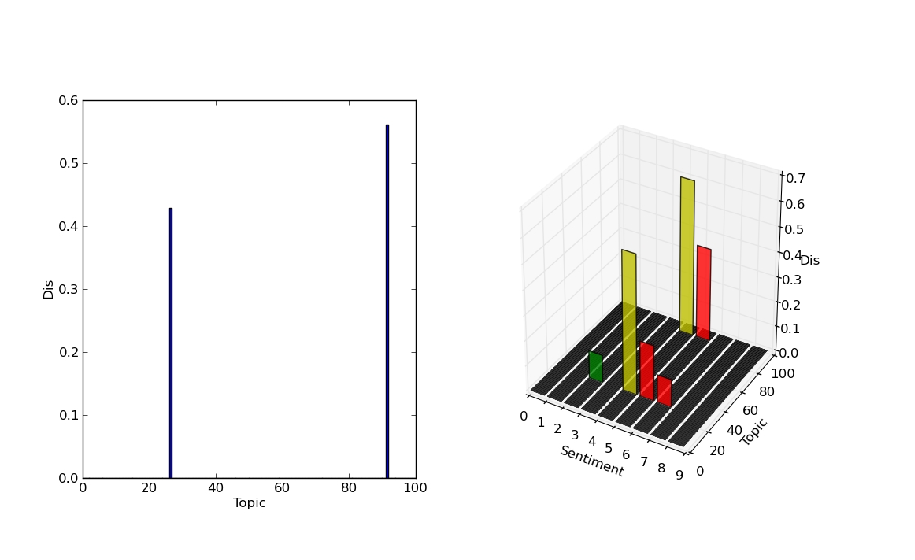
\includegraphics[width=3.5in,height=1.8in]{fig1.pdf}
\caption{Subjectivity model example. The left subgraph denotes interests distribution on topic 23 and 86: $ ( w_{u}\left( 23 \right)=0.43, w_{u}\left( 86 \right)=0.57)  $. The right subgraph denotes opinions towards two topics: $ O_{23}=( d_{u,23} \left( 2 \right)=0.1, d_{u,23} \left( 4 \right)=0.5,d_{u,23} \left( 5 \right)=0.3,d_{u,23} \left( 6 \right)=0.1) $, $ O_{86}=( d_{u,86} \left( 4 \right)=0.66, d_{u,86} \left( 5 \right)=0.34 ) $.}
\label{fig0}
\end{figure}

Specially, the topics and opinions of a tweet can also be represented by the subjectivity model in the form of  Equation~\ref{usermodel}. Therefore we assume that there is also a subjectivity model for a tweet, and will not differentiate it from the subjectivity model of a user in this paper. 
 
\subsection{Establishment of Subjectivity Model}
\label{establishment}

The definition of the subjectivity model is in an abstract form by using latent concepts of topics and opinions,  which need to be derived from the message histories of all users $ M=\lbrace M_{u}\vert u \in V\rbrace$.

\subsubsection{Topic Analysis}
\label{topic}

Topic analysis for all users in a global network on Twitter is a non-trivial task. 
There are hundreds of millions of users and billions of tweets associated with these users. The effectiveness and efficiency of the topic analysis algorithm is a challenge.
However, the follow relationship on Twitter is a strong indicator of a phenomenon called ``homophily'', which has been observed in many social networks \cite{mcpherson2001birds}.
Homophily implies that a user follows another user because of sharing common interests. 
According to the principle of homophily, we put forwards the concept of \textbf{local topic space} by combining topic analysis with network topology on Twitter: 
\begin{definition}[Local Topic Space]
\label{local}
In a global social network $G=\left( V,E \right) $, for a user $ u \in V $, we use $ G_{u}^{\tau} \subseteq G$ 
to denote $ u $'s $ \tau $-ego network, where $ \tau $-ego network means subnetwork formed by $ u $'s $ \tau $-hop 
friends in the network $ G $, and $ \tau \geqslant 1 $ is a tunable integer parameter to control the scale of the ego network. 
For the $ \tau $-ego network of $ u $, all users' interests are assumed concentrate on limited topics derived from their UGC, and these topics form a local topic space $ T_{u} $.
\end{definition}

Previous studies have tried to identify topics from tweets by finding key words \cite{chen2010short}, extracting  entities \cite{abel2011analyzing} or linking tweets to external knowledge categories \cite{macskassy2011people}. However, works show that topic model such as Latent Dirichlet Allocation (LDA) \cite{blei2003latent} is more effective in identifying topics from short and informal social media language \cite{hong2010empirical}. Therefore we adopt the user-level LDA model for topic analysis, which regards all tweets of a user as one document of LDA. The LDA model is adapted to our local topic space assumption, and the relatively tiny size and topic concentration of users in an ego network lower the impact of data sparsity, and degrade the computational difficulty of LDA. 

\subsubsection{Opinion Mining}
\label{opinion}

In the Natural Language Processing domain, opinion mining or sentiment analysis is formally defined as the computational study of sentiments and opinions about topics expressed in a text \cite{liu2012sentiment}. Opinions are often regulated as sequential discrete values to represent sentiment strength. Researches on the sentiment analysis of social media have provided effective techniques and tools \cite{thelwall2010sentiment,hu2013unsupervised}. In this work,we just make use of the off-the-shelf work, i.e. SentiStrength \cite{thelwall2010sentiment}. 
SentiStrength assigns two values to each tweet standing for sentiment strengths: a negative value within $ \left[ -5,-1 \right]  $ denoting negative strength, and a positive value within $ \left[ 1,5 \right]  $ denoting  positive strength. The $ \left[ -5,5 \right] $ sentiment valence space can be used to catch fine opinion distributions in the subjectivity model. 
For the convenience of calculation, we map the output of SentiStrength to a single value in sentiment valence space $ \left[ 0, 8 \right] $ as follows:
\begin{equation}
\label{opinionmap}
o= \left\{ 
\begin{array}{lll}
{p+3} & if \vert p \vert > \vert n \vert \\
{n+5} & \text{if } \vert n \vert > \vert p \vert \\
{4}  & \text{if } \vert p \vert = \vert n \vert
\end{array}
\right.
\end{equation}
where $ p $ denotes the positive strength and $ n $ denotes the negative strength. 

\subsubsection{Concreting Subjectivity Model}
\label{concrete}
 
As Definition~\ref{local} describes, a $ \tau $-ego network $ G_{u}^{\tau}=\left( U,E_{u} \right)  $ for a user $ u $ can be extracted from global network. 
Then the subjectivity model of each user $ u \in U $ can be concreted within the ego network. 
Let $ M_{u}$ denote tweets collection published by user $ u $, and $ M=\lbrace M_{u} |u \in U \rbrace$ denote all tweets collections of users in $ G_{u}^{\tau} $. A topic model $P\left(\theta,\beta | M \right) $ can be constructed with user-level LDA model, of which the parameter $\theta$ reprents user-topic distribution and $\beta$ reprents topic-vocabulary distribution. All topics of the topic model form a local topic space $ T_{u} $. 
The parameter $ \theta_{u} $ represents the topic distribution of user $ u $ over $ T_{u} $. Simultaneously SentiStrength is applied to each tweet $ m \in M_{u} $ and outputs sentiment strength $ s_{m} $. 
The subjectivity model $P\left( u\right)  $ is established as follows:
\begin{itemize}
\item Step 1, the parameter $ \theta_{u} $ naturally corresponds to interests distribution of user $ u $ in the local topic space $ T_{u} $, and the topics $ u $ talks about are $ Z_{u}= \left\lbrace t \vert p\left( t \vert \theta_{u}\left( t \right)  \right)>0 , t \in T_{u}\right\rbrace $.
\item Step 2, the topic model is applied to each tweet $ m $ to identify topics it talks about, denoted as $ Z_{m} =\left\lbrace t \vert p\left( t \vert \theta, \beta \right)>0 , t \in T_{u} \right\rbrace $.
\item Step 3, the opinion distribution of user $ u $ towards topic $ t \in Z_{u} $ can be calculated as: 
\begin{equation}
\label{opinionall}
O_{t}= \left\lbrace d_{u,t}\left( o\right)= \dfrac{N_{o}}{\sum_{o \in O} N_{o}} |o \in O, O=\left[ 0,8 \right] \right\rbrace 
\end{equation}
where $ N_{o} $ is the number of times user $ u $ expresses an opinion towards topic $ t $ with sentiment strength $ o $, which can be calculated as:
\begin{equation}
\label{opinion1}
N_{o}=\sum_{m \in Mu} I\left( s_{m} \right) , \text{ if } s_{m}=o \& t \in Z_{m}
\end{equation}
\begin{equation}
\label{opinion2}
I\left( s_{m} \right)=\left\{
\begin{array}{ll}
{1} & \text{if } s_{m}=o \& t \in Z_{m}\\
{0} & \text{else}
\end{array}
\right.
\end{equation}
For simplicity, it is postulated that the sentiment of each tweet $ s_{m} $ is related to all topics it talks about in $ Z_{m} $. As a future work, we will adopt more sophisticated method to identify opinion towards each topic in a tweet.
\end{itemize}

As a special case, we can also establish a subjectivity model $ P\left( m \right)  $ for a tweet $ m $ with only step 2 and 3. Note that the opinion distribution for each topic $ t $ of the tweet is $(d_{m,t}\left( s_{m}\right)= 1.0 )$. 

\section{Retweeting Analysis With Subjectivity Model}

Apart from the context constraints such as network topology, a tweet is more likely to be retweeted by a user who finds its content worth to. 
Therefore, we are not interested in modelling the tweet by itself as other researchers \cite{naveed2011searching,pfitzner2012emotional}, but understanding the underlying reasons that a user disseminates the tweet based on his subjective initiative. 
We assume that if a tweet is published by the author, all followers will read it in time. 
Under such assumption, we investigate the problem within a 1-ego network for the author of target tweet. 
In the ego network, the relations among a tweet, the author and followers are illustrated as Figure~\ref{fig1}.
\begin{figure}[htb]
%\setlength{\belowcaptionskip}{-0.2cm} 
\centering
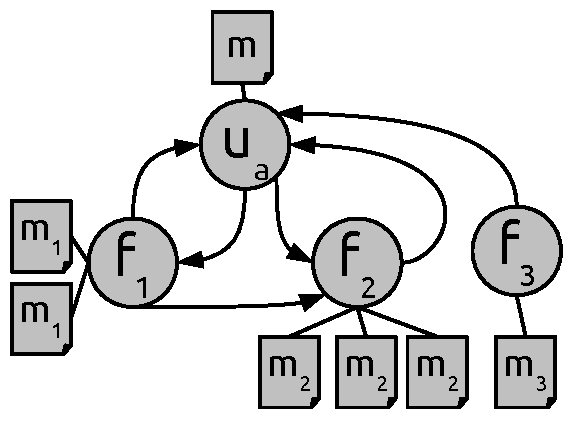
\includegraphics[width=1.5in,height=1.1in]{ego.pdf}
%\vspace{-4em}
\caption{Illustration of relations among tweet, author and followers. Author is denoted as $ u_{a} $, tweet as $ m $, followers as $ f_{i} $ and tweets of follower $ f_{i} $ as $ m_{i} $. An directed edge $ \left( f_{i},u_{a} \right)  $ means that $ f_{i} $ is exposed to the messages published by $ u_{a} $.}
\label{fig1}
\end{figure}

\subsection{Problem Formulation}
\label{formulation}

The retweeting analysis problem can be formulated as following:
For a target tweet $ m $, let $ F $ denote the followers who receive $ m $ by following its author $ u_{a} $, and for each user $ u \in F \cup \left\lbrace u_{a} \right\rbrace  $, let $ M_{u} $ denote a tweet collection $ u $ has published. 
For each follower $ u \in F $, we can define a quadruple $ <u, u_{a}, m, r_{f}>  $: 
\begin{itemize}
\item $ r_{f} $ is a binary label indicating if $ m $ is retweeted by $ u $.
\item Firstly our work focuses on building subjectivity model $ P\left( u \right)  $ for each user $ u \in F \cup \left\lbrace u_{a} \right\rbrace $ in the ego network with all tweets collections $ M=\left\lbrace M_{u} | u \in F \cup \left\lbrace u_{a} \right\rbrace  \right\rbrace  $.
\item Then we investigate the relation between the subjectivity of a user and his retweeting behavior to predict $ r_{f} $ by calculating subjectivity similarities between tweet $ m $, its author $ u_{a} $ and follower $ u $. 
\end{itemize}

\subsection{Subjectivity Similarity}
\label{similarity}

It is assumed that if a tweet is similar enough with the subjectivity of a user in terms of topics and opinions, the user will have a very high probability to decide to retweet it. 
With the subjectivity models estabilshed for the users and tweet, the subjective decision-making process can be simulated by calculating the subjectivity similarity between the tweet and users. 
In this section, we define a novel similarity measurement to quantify the subjectivity similarity, which consists of topic similarity and opinion similarity. 
 
\subsubsection{Topic Similarity}
\label{topsim}

The similarity between two topic distributions can be calculated with methods such as the cosine distance \cite{cha2007comprehensive} or the Jensen-Shannon Divergence \cite{weng2010twitterrank}.
We adopt the cosine distance to measure the topic similarity because it performs better than other measurements in our research settings. It is defined as:
\begin{equation}
sim_{topic}=\dfrac{\theta_{m} \cdot \theta_{u}}{\parallel \theta_{m} \parallel \parallel \theta_{u} \parallel}
\end{equation}
where $ \theta_{u}$ denotes the topic distribution of user $ u $ and $\theta_{m}$ denotes the topic distribution of tweet $ m $. 

\subsubsection{Opinion Similarity}
\label{opsim}

Opinion in the subjectivity model is treated  as a distribution over sentiment valence space with each entry of the distribution representing the proportion of the corresponding value in the overall sentiment values. 
However, values in the sentiment valence space are not independent. 
They are sequential and represent strength of the sentiment. Illustrated as Table~\ref{tab1}, opinion $ O_{t}^{1} $ is the most negative towards topic $ t $ (100\% of strength value 0), while opinion $ O_{t}^{2} $ (100\% of strength value 7) and $ O_{t}^{3} $ (100\% of strength value 8) are both positive.
If the cosine similarity measurement is adopted to calculate opinion similarity, all similarities among them are 0.
In fact $ O_{t}^{2} $ is more similar with $ O_{t}^{3} $ than $O_{t}^{1} $ because they both hold positive opinion and their sentiment distance is much less than $ O_{t}^{1} $.  
Therefore, opinion similarity can't be calculated simply as the topic distributions. 
To accurately catch opinion similarity, we propose a novel method by combining both sentiment distance and distribution similarity.
The opinion similarity between two opinions on the same topic $ t $ can be calculated as: 
\begin{equation}
\label{opinionsim}
sim_{opinion}^{t}(O_{t}^{1},O_{t}^{2})=\dfrac{8-|\sum_{i=0}^{8}d_{i}^{1}v_{i}-\sum_{i=0}^{8}d_{i}^{2}v_{i}|}{8}
\end{equation}
where $ d_{i} $ denotes the $ i^{th} $ entry of opinion distribution vector, and $ v_{i} $ denotes corresponding sentiment strength value. 
\begin{table}[t]
\scriptsize
\centering
\caption{Illustration of opinion similarity}
\label{tab1}
\begin{tabular}{|l|l|l|l|l|l|l|l|l|l|}
\hline
 & 0 & 1& 2 & 3 & 4 & 5 & 6 & 7 & 8 \\
\hline
$O_{t}^{1}$ & 1.0 & 0.0 & 0.0 & 0.0 & 0.0 & 0.0 & 0.0 & 0.0 & 0.0 \\
\hline
$O_{t}^{2}$ & 0.0 & 0.0 & 0.0 & 0.0 & 0.0 & 0.0 & 0.0 & 1.0 & 0.0 \\
\hline
$O_{t}^{3}$ & 0.0 & 0.0 & 0.0 & 0.0 & 0.0 & 0.0 & 0.0 & 0.0 & 1.0 \\
\hline
\end{tabular}
\end{table} 
The similarities of opinions in Table~\ref{tab1} calculated with Equation~\ref{opinionsim} are $ sim(O_{t}^{1},O_{t}^{3})=0 $, $ sim(O_{t}^{2},O_{t}^{3})=7/8 $ and $ sim(O_{t}^{1},O_{t}^{2})=1/8 $, which are consistent with intuitive understanding. 

Accordingly, overall opinion similarity between two subjectivity models can be calculated as normalized similarity of all opinion similarities on common topics. 
\begin{equation}
sim_{opinion}(u_{1},u_{2})=\dfrac{\sum_{t=1}^{|T|}sim_{opinion}^{t}(O_{t}^{1},O_{t}^{2})}{|T|}
\end{equation}
where $ T $ denotes the common topics between two subjectivity models, which can be regarded as the intersection between their topic sets $ Z_{u_{1}} $ and $ Z_{u_{2}} $ described in the section of subjectivity model establishment. 

\subsubsection{Subjectivity Similarity}

By combining topic similarity and opinion similarity, the subjectivity similarity can be defined as follows:
\begin{equation}
\label{subsim}
Sim_{sub} \left( m,u \right) = \lambda * sim_{topic}+\left( 1-\lambda \right)*sim_{opinion}
\end{equation}
where $ \lambda $ is the coefficient used to control the proportions of topic similarity and opinion similarity in the holistic subjectivity similarity. 
A user cares more about topics with a larger $ \lambda $, and cares more about opinions with a samller $ \lambda $. 
A personalized $ \lambda $ can be learned from the retweeting history of a user, which enable us to catch subtle retweeting habit and improve retweeting prediction performance for each user. 

\subsection{Retweeting Analysis}
\label{analysis}

The motivation of retweeting behavior is complicated, which involves the target tweet, its author and followers who is following its author, with their relations illustrated as Figure~\ref{fig1}. 
The idea behind this work is that taking opinions towards interests into account can yield benefits in explaining the subjective motivation of retweeting behavior. 
Specifically, given a tweet $ m $, the author $ u_{a} $ and any one of the followers $ u $, we consider the probability of user $ u $ to rewteet $ m $ from three aspects: 
(i) how similar is the tweet $ m $ to the subjectivity of user $ u $ in terms of topics and opinions, i.e. $ sim_{sub} \left( m,u \right) $, (ii) how like-minded are the author $ u_{a} $ and user $ u $ considering their similarity of subjectivity, i.e. $ sim_{sub}\left( u_{a},u \right) $, and (iii) how original is the tweet $ m $ judged from its similarity with the subjectivity of its author $ u_{a} $, i.e. $ sim_{sub}\left( m,u_{a} \right)  $. 
From the point of motivation, a user might retweet a message if its content is approximate to his subjectivity, its author is a like-minded friend and it is original from inner subjectivity of its author. 
In next section we carry out a set of experiments to inspect and verify the impact of such motivation on retweeting behavior. 

\section{Experiments}
\label{experiments}

\subsection{Dataset and Settings}
We adopt the Twitter dataset of previous work \cite{Luo:2013RMF}. 
To form the dataset, 500 target English tweets published from September 14th, 2012 to October 1st, 2012 were monitored to find who would retweet it in the next days. 
Besides, each target tweet was set as starting point to collect at least 200 historical tweets for its author and followers.
Overall, there are 3,0876 users who have retweeted at least 20 times in their historical tweets, 5214 of which retweet at least one target tweet during the monitored period. To avoid the bias introduced by dataset imbalance, an evaluation dataset was constructed by taking 5,214 retweeters as positive instances, and randomly sampling 5,214 non-retweeters as negative instances. All users in the evaluation dataset were separated into the 1-ego network of their target tweet's author to establish their subjectivity model. 
For subjectivity similarity, a \textit{mini-batch gradient descent} algorithm was implemented to optimize the coefficient $ \lambda $ in Equation~\ref{subsim} for each user with his retweeting history. Therefore, all $ \lambda $s of three subjectivity similarities ($ sim_{sub} \left( m,u \right) $, $ sim_{sub}\left( u_{a},u \right)  $, $ sim_{sub}\left( m,u_{a} \right)  $) were optimized to reflect the personalized retweeting habit. As a result, the optimized $ \lambda $s are used to calculate three subjectivity similarities for each user of the evaluation dataset with their own target tweets, which are used to study their retweeting behaviors.

\subsection{Correlation Test}

First of all we want to assess the existence of a correlation between subjectivity similarity and retweeting behavior. 
To verify such correlation, a statistical hypothesis test called Analysis of Variance (ANOVA) \cite{fisher1970statistical} is used. 
ANOVA tests the \textit{null hypothesis} that samples in two or more groups are derived from the same population by estimating the variance of their means. 
This test fits our goal of testing whether the retweeters and non-retweeters have the same subjectivity similarity means. 
ANOVA test produces two output values: the \textit{F-ratio} and the \textit{p-value}. 
If the difference between the means is due to chance, the expected value of the \textit{F-ratio} is 1.00, otherwise it is larger than 1.00. 
If the p-value is lower than the significance level $ \alpha $, the \textit{null hypothesis} is rejected, which means the results is considered statistically significant. 
The significance level is conventionally used at 0.01.
At the same time, we carry out the test by varying the topic number of LDA for topic analysis as 50, 100, 150 and 200 to determine the impact of topic number. 
The results are listed in Table~\ref{tab2}, The bold-faced entries mean that the \textit{p-value} is lower than significance level $ \alpha = 0.01 $.
\begin{table}[htb]
\scriptsize
\centering
\caption{ANOVA results for subjectivity similarities}
\label{tab2}
\begin{tabular}{|c|c|c|c|c|}
\hline
\multicolumn{2}{|c|}{Similarity}& $ sim_{sub} \left( m,u \right) $ & $ sim_{sub}\left( u_{a},u \right)  $ & $ sim_{sub}\left( m,u_{a} \right)  $\\
\hline
\multirow{2}{*}{50} & \textit{F} & \textbf{12.182} & 2.212 & 4.236 \\
\cline{2-5}
  & \textit{p} &  $\mathbf{4.44e^{-06}}$  & 0.140 & 0.272\\
\hline
\multirow{2}{*}{100} & \textit{F} & \textbf{43.892} & \textbf{31.145} & \textbf{28.466} \\
\cline{2-5}
  & \textit{p} &  $\mathbf{8.65e^{-11}}$  & $\mathbf{3.55e^{-08}}$ & $\mathbf{1.32e^{-09}}$\\
\hline
\multirow{2}{*}{150} & \textit{F} & \textbf{22.356} & \textbf{12.240} & \textbf{14.664} \\
\cline{2-5}
  & \textit{p} &  $\mathbf{2.43e^{-08}}$  & $\mathbf{6.25e^{-06}}$ & $\mathbf{8.46e^{-07}}$\\
\hline
\multirow{2}{*}{200} & \textit{F} & \textbf{31.675} & \textbf{20.616} & 6.145\\
\cline{2-5}
  & \textit{p} &  $\mathbf{4.22e^{-06}}$  & $\mathbf{2.92e^{-05}}$ & 0.26\\
\hline
\end{tabular}
\end{table}

Note that for the topic numbers of 100 and 150, all similarities yield \textit{p-values} below $ \alpha $ with \textit{F-ratio} above 1.00. This suggests that the subjectivity similarities could be useful features for modeling retweeting behavior. 
For the rest experiments, we set the topic number as 100 for LDA model. 

\subsection{Performance Evaluation}

To evaluate the performance of retweeting behavior prediction, we firstly compare our model against other topic-based models including TF-IDF model (modelling user interests with bag-of-words), entity-based model (modelling user interests with entities extracted from the UGC) and hashtag-based model(modelling user interests with hashtags used in the UGC) \cite{abel2011analyzing}. The cosine distance is used as similarity measurement for these models as topic similarity in our model for comparison.

In addition, subjectivity model tries to catch the subjective motivation of users based on their UGC, whereas other important factors associated with retweeting behavior are not considered, such as network topology and metadata of users. 
Therefore, our model is also compared with the method of Luo \emph{et al.}~\shortcite{Luo:2013RMF} (marked as ``LUO''), in which diffenent factors that might affect rewteeting behaviors have been considered.
In their work they use four feature families: ``Retweet History''(follower who have retweeted a user before is likely to retweet again), ``Follower Status''(the number of tweets, followers, friends, listed times and verified state), ``Follower Active Time''(interaction with other users) and ``Follower Interests''(TF-IDF bag-of-words model for user interests). 
Based on the results of Comparative experiment, we also carry out combining experiments to demonstrate that performance of their method can be improved by using our model instead of bag-of-words model. 
\begin{table}[h]
\scriptsize
\centering
\caption{Accuracy performance. A significant improvement over baseline with $ \ast $ and LUO' model with $ \ddagger $ ($p < 0.05$).}
\label{tab3}
\begin{tabular}{|l|l|l|l|}
\hline
Feature & Accuracy(\%) & Feature & Accuracy(\%)\\
\hline
RB & 60.85 & & \\
TF-IDF & 62.85   $\ast$ & LUO & 71.76 $ \ast  $\\
entity & 68.76  $\ast$ & LUO+entity & 72.15 $\ast$\\
hashtag & 59.12  & LUO+hashtag & 68.44 $\ast$\\
$ sim_{sub} \left( m,u \right) $ & 73.88   $\ast  \quad \ddagger $ &LUO+$ sim_{sub} \left( m,u \right)$ & 74.04  $ \ast \quad \ddagger $\\
$ sim_{sub}\left( u_{a},u \right)  $ & 70.04   $\ast  $ & LUO+$ sim_{sub}\left( u_{a},u \right)$ & 70.27  $ \ast $\\
$ sim_{sub}\left( m,u_{a} \right)  $ & 69.64   $\ast  $ & LUO+$ sim_{sub}\left( m,u_{a} \right)$ & 71.86  $ \ast $\\
$ sim_{all}  $ & \textbf{75.64}   $\ast \quad \ddagger $ & LUO+$ sim_{all}  $ & \textbf{78.15}  $ \ast \quad \ddagger $\\
\hline
\end{tabular}
\end{table}

The evaluation dataset is randomly divided into five parts for 5-fold cross-validation. 
The logistic regression classifier of Scikit-learn machine learning package \cite{scikit-learn} is used for training and testing.
It is noted that followers who previously had a history of retweeting might do this in the future, so we set a baseline (marked as ``RB''), which simply predicts users who have retweeted the author previously as the retweeters of target tweet. 
The accuracy is taken as our evaluation metric, and the results are listed in Table~\ref{tab3}, in which the compariative results are listed in the left part and the combining results in the right part.

Firstly, all models except the hashtag-based model outperform the baseline (60.85\%) significantly. While for hashtag-based model, its accuracy is the lowest (59.12\%), the reason might lie in a very low usage of hashtag in a user's tweets. 

Secondly, in the comparative results, $ sim_{sub} \left( m,u \right) $ and $ sim_{all}  $ outperform ``LUO'' (71.76\%) significatantly.
The best performance is achieved by the $ sim_{all}  $ (75.64\%), for which we feed all three subjectivity similarities into the logistic classifier to test the impact of their combination. 
The perfromance of TF-IDF model (62.85\%) is only better than baseline. 
The entity-based model (68.76\%) is very close to  $ sim_{sub}\left( u_{a},u \right)$ (70.04\%) and $ sim_{sub}\left( m,u_{a} \right)  $ (69.64\%), and the difference is not significant.

Finally, in the combining evaluation experiment, for which the TF-TDF model of ``LUO'' feature set is replaced with other models, the results are diverse. $ sim_{sub} \left( m,u \right) $ gives a significant improvement (LUO+$ sim_{sub} \left( m,u \right) $, 2.12\% improvement) over ``LUO'', but other two subjectivity similarities and the entity-based model can not improve performance significantly. The performance is even degraded after combining with the hashtag-based model. 
But noticing that, the most significant improvement(LUO+$ sim_{all}  $, 6.39\% improvement) is achieved by combining with all subjectivity similarities. 

The results above show that subjectivity model can better help predicting retweeting behavior than other models and can be regarded as a better way to model the users for retweeting behavior analysis. 


%\subsection{Case Study}
%\label{example}
%In this section we give a vivid description about the subjectivity model and its ability in explaining the retweeting behavior with an example. 
%The topic and opinion of one target tweet, subjectivity models for its author, and two followers (one retweet it while the other does not) are shown as Figure~\ref{fig2}. 
%The right part of each sub-figure illustrates topic distribution and the left part illustrates opinion distribution. 
%It is clear that the tweet talks about the 14th topic of the local topic space. 
%\begin{figure*}[htb]
%%\setlength{\belowcaptionskip}{-0.2cm} 
%\centering%,bb=0 0 1280 960
%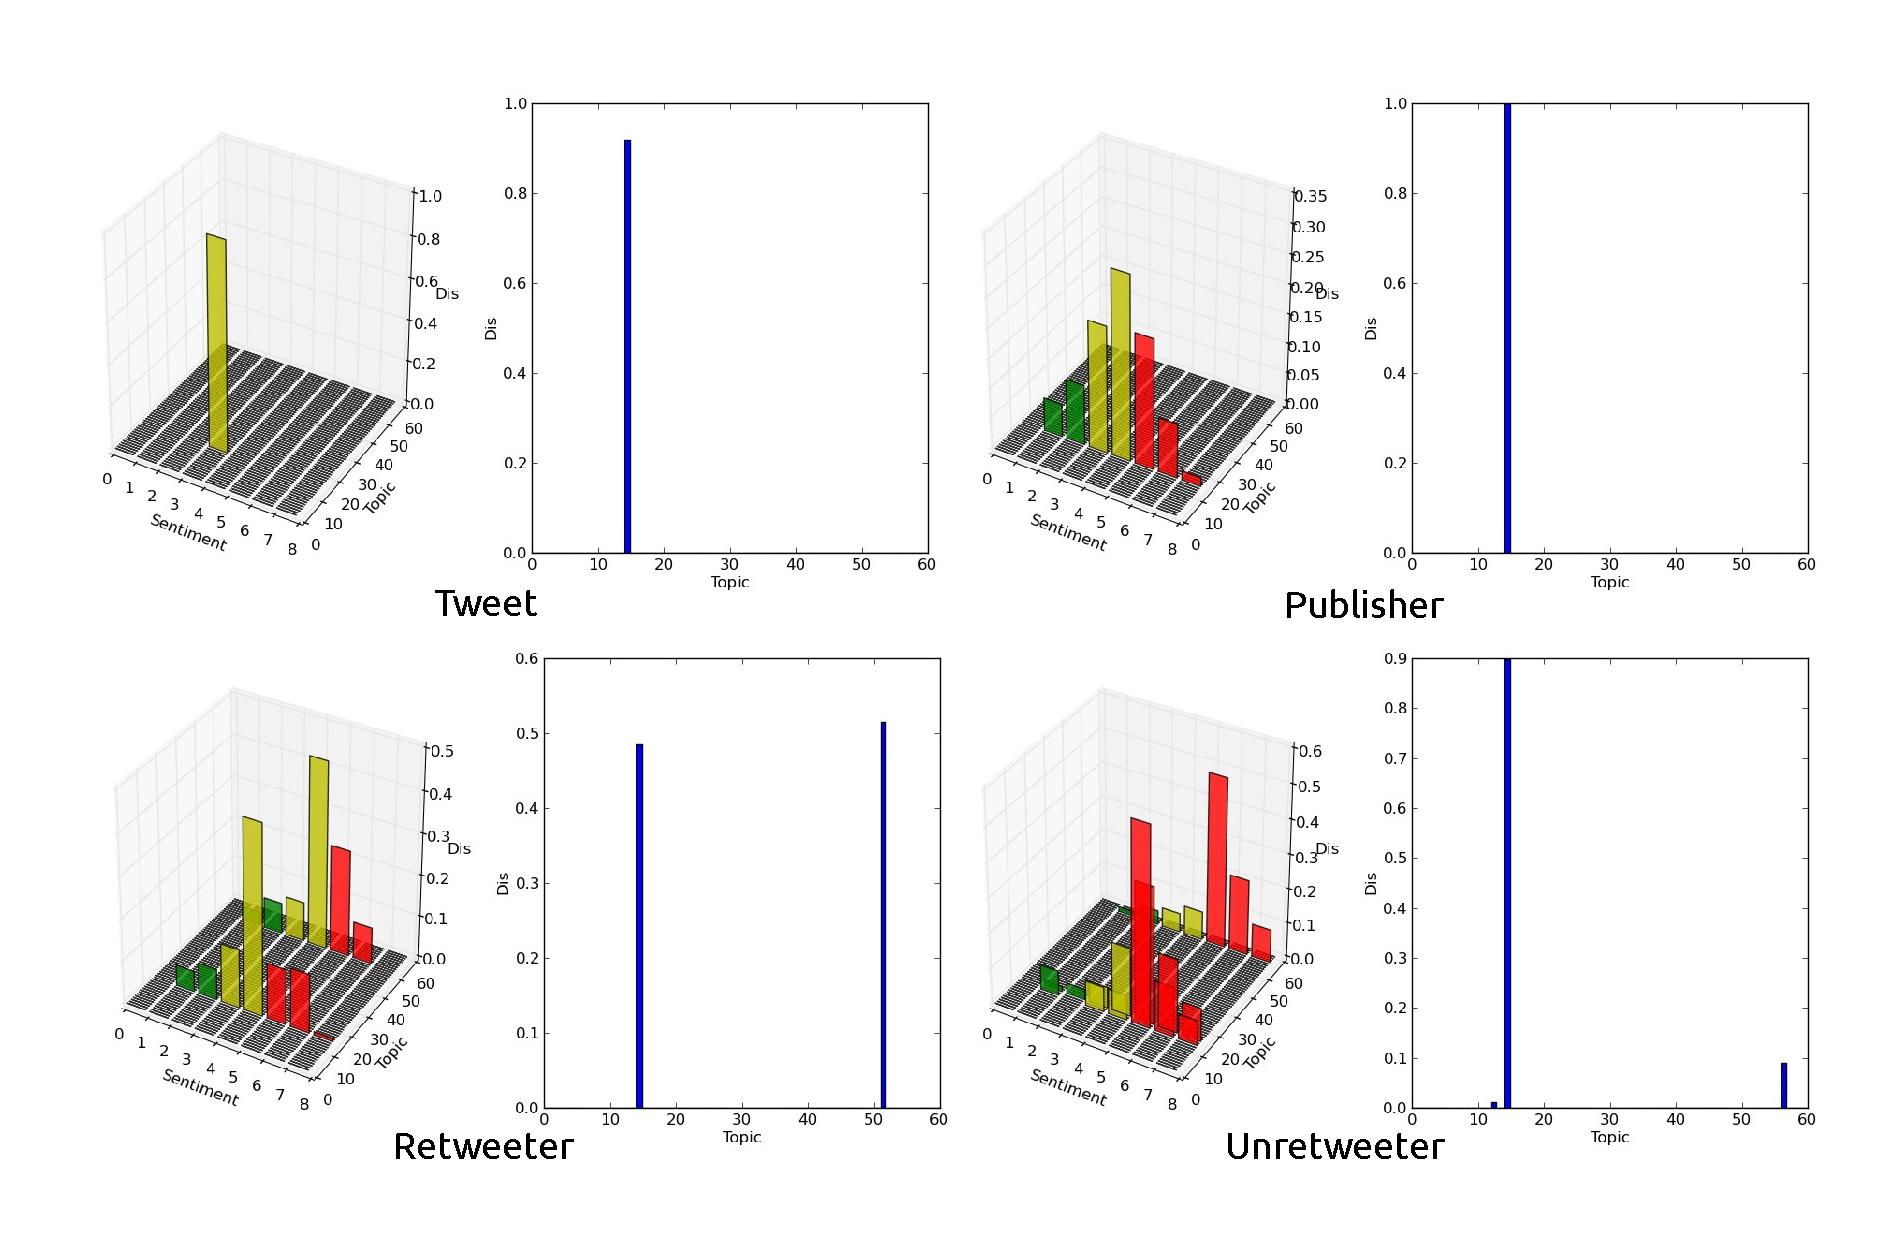
\includegraphics[width=6.0in,height=3.5in]{tweets10.pdf}
%%\vspace{-4em}
%\caption{subjectivity model examples.}
%\label{fig2}
%\end{figure*}
%Figure~\ref{fig3} shows top words of the 14th topic, the tweets of author and followers with word cloud\footnote{We use TagCrowd (\url{http://tagcrowd.com/}) to produce word cloud.}.
%\begin{figure}[htb]
%%\setlength{\belowcaptionskip}{-0.2cm} 
%\centering
%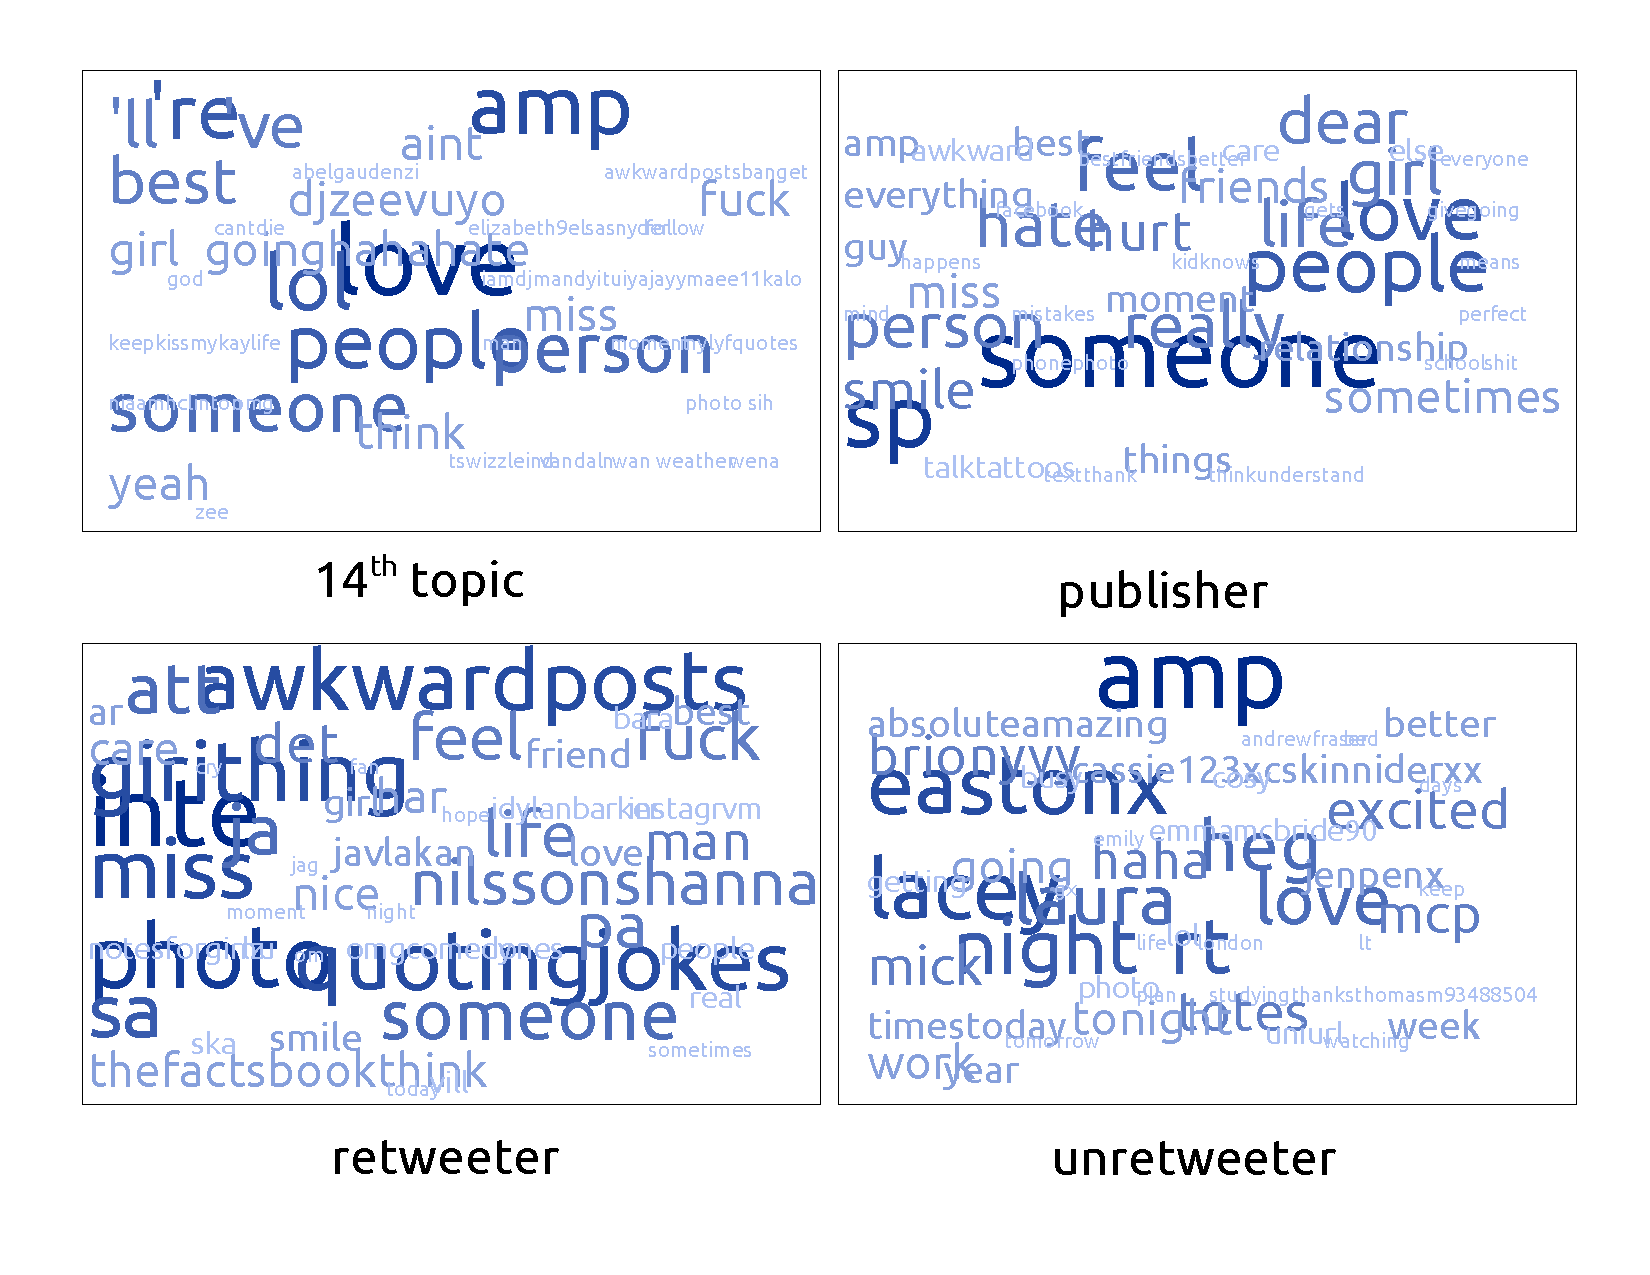
\includegraphics[width=3.5in,height=2.2in]{text_cloud.pdf}
%%\vspace{-3em}
%\caption{Word cloud of 14th topic, publisher and followers}
%\label{fig3}
%\end{figure}
%Content of the tweet is:\\
%\textit{Tweet: ``Sometimes the right person for you was there all along. You just didn't see it because the wrong one was blocking the sight''} \\
%The topic of this tweet is about ``love between people'' and the opinion is neutral, which is in accordance with the 14th topic word cloud in Figure~\ref{fig3} and sub-figure of tweet in Firgure~\ref{fig2}.
%The author concentrates on the 14th topic, and his opinions are mainly neutral (as Figure~\ref{fig2},~\ref{fig3} show).
%As for two followers, the ``retweeter'', has published tweets about two topics (the 14th and 52nd topic) uniformly and his opinions towards the two topics are mainly neutral.
%While the ``unretweeter'', has also talked about two topics (14th and 56th topic), but he is mainly interested in 14th topic and has positive opinion.
%Although two followers have same interest (the 14th topic), their different opinions elicit their different decisions, which verify the subjectivity model can help better understand the retweeting motivation by modelling not only topics but opinions.

\section{Related Work}
\label{relatedwork}
   
User modelling provides insights into user's online behaviors. 
Hannon \emph{et al.}~\shortcite{hannon2010recommending} proposed that users can be modeled by tweets contents and the relation of social networks, while content-based model can find similar users who are "distant" without following relations. 
Macskassy and Michelson~\shortcite{macskassy2011people} discovered user interests by leveraging Wikipedia as external knowledge to determine a common set of high-level categories that covers entities in tweets. 
Ramage \emph{et al.}~\shortcite{ramage10microblogs} made use of topic models to analyze tweet contents at the level of individual, showing improved performance on tasks such as post filtering and user recommendation. 
Xu \emph{et al.}~\shortcite{xu2012modeling} proposed a mixture model which incorporated three important factors, namely breaking news, friends' timeline and user interests, to explain user posting behavior.
Pennacchiotti and Popescu~\shortcite{pennacchiotti2011machine} proposed a most comprehensive method to model Twitter users for user classification, confirming the value of in-depth features by exploiting the UGC. 
A large body of studies have analyzed characteristics of retweeting \cite{macskassy2011people,Luo:2013RMF}, examining factors that lead to increased retweetability \cite{suh2010want,comarela2012understanding} and designing models to estimate the probability of being retweeted \cite{petrovic2011rt,jenders2013analyzing,pfitzner2012emotional}. However, all of the above works neglect the subjectivity of users, which is the underlying reason for the decision-making of subjective initiative individuals. We have fisrtly proposed a novel subjectivity model for retweeting behavior analysis. 

\section{Conclusion}
In this paper, from the point of motivation, we postulate that the online behaviors of social media users are affected by their subjectivity. Therefore, a novel subjectivity model has been proposed by combining topics and opinions to model the subjectivity of users. Also an algorithm has been designed to establish the subjectivity model. To make the algorithm more efficiently, only the users of an ego network are considered and a local topic space is proposed according to the homophily principle. A novel subjectivity similarity measurement has been put forward in terms of topic simlarity and opinion similarity. The subjectivity model is applied to the retweeting analysis with three subjecivity similarities among tweets, authors and followers. 
Experiment results demonstrate the effectiveness of the proposed model in the retweeting analysis problem and show that subjectivity model is able to reach better understanding of retweeting behavior. 

In the future, we will apply the subjectivity model to other social network analysis task such as link prediction and friend recommendation. 

\bibliography{subjectivity}
\bibliographystyle{aaai}
\end{document}
